\begin{itemize}
\item Ahmad Syafrizal Huda (1164062)
\item Annisa Fathoroni (1164067)
\item Puad Hamdani (1164084)
\item Rahmi Roza (1164085)
\item Tasya Wiendhyra (1164086)
\end{itemize}

\section{Definisi RESTful Web Service}
REST merupakan salah satu macam web service yang memasukkan konsep perpindahan antar state. State disini bisa dibayangkan seperti jika browser meminta suatu halaman web, maka server akan mengirimkan state halaman web yang sekarang ke browser. Menurut salah satu perkembangan Tidwell, D., 2001 bernavigasi melalui link-link yang disediakan sama halnya dengan mengganti state dari halaman web. Begitu pula REST bekerja, dengan bernavigasi melalui link-link HTTP untuk melakukan aktivitas tertentu, seakan-akan terjadi perpindahan state satu sama lain \cite{indrawan2017implementasi}.

\section{Prinsip atau Karakter Pada RESTful}
RESTful adalah salah satu teknologi web service untuk membuat suatu sistem yang terdistribusi dimana cara kerjanya berdasarkan resource. RESTful sendiri merupakan software yang didesain untuk penekanan pada skalabilitas,kesederhanaan dan kegunaan. Metode dalam REST terdiri dari empat prinsip utama teknologi, yaitu \cite{aji2016penerapan}:
\begin{enumerate}
\item Resource identifier melalui Uniform Resource Identifier (URI), REST Web service mencari sekumpulan sumber daya yang mengidentifikasi interaksi antar klien.
\item Uniform interface, sumber daya yang dimanipulasi CRUD (Create, Read, Update, Delete) menggunakan operasi PUT, GET, POST, dan DELETE.
\item Self-descriptive messages, sumberdaya informasi tidak terikat, sehingga dapat mengakses berbagai format konten (HTML, XML, PDF, JPEG, Plain Text dan lainnya). Metadata pun dapat digunakan.
\item Stateful interactions melalui hyperlinks, setiap interaksi dengan suatu sumber daya bersifat stateless, yaitu request messages tergantung jenis kontennya.
\end{enumerate}

\section{Contoh-Contoh Penerapan  RESTful}
\subsection{Implementasi RESTful Web Service untuk Sistem Penghitungan Suara Secara Cepat pada Pilkada}
Metode ini yang digunakan oleh penyelenggara pemilihan umum untuk menentukan hasil pilkada. Dengan memanfaatkan teknologi yang ada, proses pengumpulan data hasil perolehan suara bisa dilakukan dengan lebih cepat. Salah satu metode baru yang bisa digunakan untuk melakukan proses tersebut adalah metode perhitungan cepat riil. Metode ini memanfaatkan teknologi informasi dan komunikasi untuk melakukan proses penghitungan suara. Real-quick count mengambil hasil perhitungan dari semua tempat pemungutan suara (TPS). Tetapi hasil tersebut dikirim langsung dari TPS ke lembaga penyedia informasi hasil perhitungan cepat, tidak melalui prosedur seperti pada real count yang mengharuskan pengumpulan data berjenjang, oleh karena itu waktu yang dibutuhkan untuk memperoleh semua hasil suara bisa dioptimalkan. Pada jurnal ini dilakukan perbandingan antara SOAP dan REST pada aplikasi mobile dan multimedia conference. Hasil penelitian yang dilakukan pada aplikasi mobile computing menunjukkan bahwa ukuran pesan pada RESTful web service mencapai 9 sampai 10 kali lebih kecil dibandingkan ukuran pesan dari web service berbasis SOAP \cite{rofiq2017implementasi}.

\subsection{Implementasi RESTful untuk Sales Order dan Sales Tracking Berbasis Mobile}
Bagian penjualan merupakan bagian yang paling penting dalam penjualan produk. Perusahaan membutuhkan sistem yang dapat membantu aktivitas dan pemesanan produk. dengan membuat sebuah Controller terlebih dahulu,yang berperan untuk menentukan informasi apa yang akan disampaikan pada saat client mengakses web service. Dibuat dengan arsitektur REST dengan menggunakan method yang di dukung protokol HTTP seperi method DELETE, UPDATE, CREATE,dll. Aplikasi mobile ini akan menggunakan data dari GPS untuk memastikan lokasi penjual juga dilengkapi barcode untuk mempercepat input data barang \cite{kurniawan2015implementasi}.

\subsection{Implementasi REST Web Service Pada Aplikasi Pengolah Pesan Yahoo Messenger Pada CV. MELIANA PRATAMA}
Mengimplementasikan REST Web Service pada aplikasi pengolah pesan Yahoo Messenger (YM). Aplikasi REST Web Service dapat dijadikan sebagai miidleware antara aplikasi pengolahan pesan Yahoo Messenger (YM) dengan database, sehingga proses transaksi ke database menjadil lebih efisien. Hal ini dikarenakan aplikasi client tidak perlu mengetahui database apa yang digunakan oleh server \cite{ikrom2015implementasi}.

\subsection{Implementasi RESTful Web Service Pada Aplikasi Iklan Baris Online}
Pada implementasi aplikasi ini menerapkan restful web service yang dimana server akan berinteraksi dengan client pada interface yang sama atau seragam. Server akan meng-host resource sedangakn client akan menjadi konsumen dari resource yang disediakan server. Pada saat server meminta atau request data script request akan dikirim dari client ke server berbentuk alamat url yang kemudian memanggil file PHP yang mengakses data dari databse server. saat pengambilan data, client akan memanfaatkan API yang terdapat dalam server. Setelah mendapat data dari client, server kemudian akan menyebar informasi yang dibutuhkan berupa kebutuhan barang/jasa yang bersangkutan kepada member atau client \cite{fauziah2014aplikasi}.

\section{Pengembangan Sistem Informasi RESTful Web Service}
Pengembangan sistem informasi kependudukan berbasis mobile dan restful pada web service yaitu\cite{kurniawati2016pengembangan}:
\begin{enumerate}
\item REST Web Service pada tahap ini akan dibuat web service yang diletakkan pada server pusat untuk mengolah data JSON. Web service memiliki 3 method yaitu json decode yaitu untuk parsing data masukan, StoreData dan json encode parsing untuk data keluaran. Parameter masukan dari database SQLite ke MySQL tampak pada gambar 5, akan diparsing ke dalam format Array. StoreData yang berhubungan langsung dengan database dalam proses input, status gagal atau sukses akan disimpan dalam Array dan diolah lagi menjadi format JSON sebagai keluaran dari web service.
\item Aplikasi Android Antarmuka aplikasi android saat dijalankan akan muncul form login. Pengguna aplikasi yaitu kepala lingkungan memasukkan username dan password kemudian tekan tombol login
\end{enumerate}

\begin{figure}[ht]
\centerline{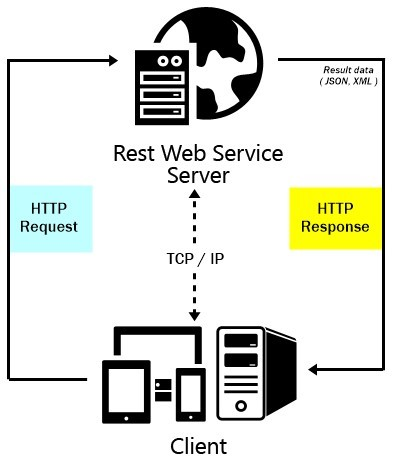
\includegraphics[width=1\textwidth]{figures/1restful.JPG}}
\caption{RESTful}
\label{labelgambar}
\end{figure}
Pada gambar \ref{labelgambar} menerangkan cara Rest Web Service melakukan request kepada server kemudian server membalasnya dengan result berupa json. Metode tersebut telah dikembangkan oleh Roy Thomas Fielding dalam disertasinya tentang Architectural Style.  Dalam disertasinya tersebut REST (Representational state transfer) didefinisikan sebagai suatu gaya arsitektur perangkat lunak untuk pendistribusian sistem hypermedia seperti WWW \cite{rofiq2017implementasi}.

\section{Implementasi Protokol OAuth 1.0 Sebagai Autentikasi pada Aplikasi SMS Blast Berbasis Android}
Sebuah aplikasi SMS Blast berbasis Android dan sebuah web service yang digunakan oleh aplikasi untuk melakukan request terhadap data nomor telepon terhadap data yang sudah ada. OAuth menggunakan token pada setiap request. Web service akan membangkitkan token yang berbeda pada setiap request dari consumer. Penggunaan token ini dapat meminimalkan kemungkinan terjadinya serangan Man in the Middle Attack dan Hijacking Attack
\cite{saputra2017implementasi}

\section{IMPLEMENTASI RESTFUL WEB SERVICE ONE CHIP MULTI-CLIENT UNTUK MENGOPTIMALKAN PENJUALAN PULSA ALL OPERATOR}
One  Chip  All  Operator adalah sebuah chip untuk pengisian pulsa kesemua operator selluler GSM dan CDMA bahkan juga dapat digunakan untuk pengisian pulsa listrik atau listrik prabayar. Chip atau kartu perdana  yang  digunakan bukan kartu Khusus atau tidak harus dipesan kedealer penyedia pelayanan pengisian pulsa,Chip yang   digunakan cukup perdana biasa,jadi nomor  yang dipakai sehari-hari dapat dijadikan sebagai chip untuk pengIsian pulsa ke semua operator. Proses awal yang dilakuakanya itu peses deployment restful  web  service. Deployment  restful web service  merupakan proses menjalankan web service pada server seperti apache tomcat agar aplikasi client dapat mengakses service database\cite{indrawan2017implementasi}.






